%adding TAIGA|Tunka data

% 11. Присоединение данных TAIGA (Tunka-133, HiSCORE) (как идея)
%         отличие тунки от каскада, черенки/сцинтиляторы
%         картинки с хмах
%         мэппинг данных
%
%         разделение гамма/кр тунка133 +

\begin{frame}{Tunka-133 and TAIGA-HiSCORE}
\begin{minipage}[c]{0.49\textwidth}
\begin{itemize}
  \item Similarities to KASCADE:
  \begin{itemize}
    \item located at the same latitude;
    \item measure the same CR spectrum;
    \item rely on the same hadronic interaction models for the interpretation of their data;
  \end{itemize}
  \item Differences with KASCADE:
  \begin{itemize}
    \item The experiments have different observation levels;
    \item They are using different measurement techniques, namely scintillator arrays and air Cherenkov detectors respectively;
  \end{itemize}
\end{itemize}
\end{minipage}
\hfill
\begin{minipage}[c]{0.5\textwidth}
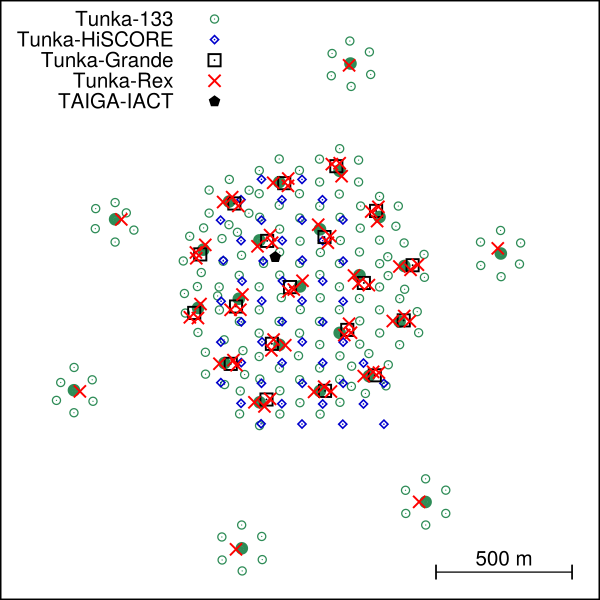
\includegraphics[width=1\textwidth]{pics/taiga_map.png}
\end{minipage}

% \vspace{1ex}
% A comparison of the cosmic-ray energy scales of Tunka-133 and
% KASCADE-Grande via their radio extensions Tunka-Rex and LOPES
\end{frame}

\begin{frame}{KASCADE-TAIGA joint analysis}
\small
The possibility to map Tunka-133 and KASCADE-Grande spectra was shown at: W.D.~Apel et al., \textit{Tunka-Rex and LOPES Collaborations}, Phys.\ Lett.\ B \textbf{763} (2016) 179
\begin{center}
    \begin{minipage}{0.50\textwidth}
        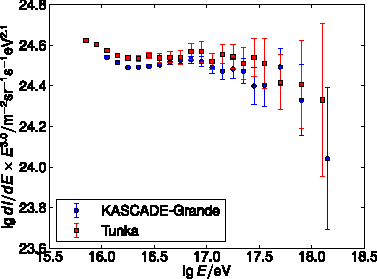
\includegraphics[width=1\textwidth]{pics/KG_tunka133_scales.pdf}
    \end{minipage}
     $\longleftarrow$~
\begin{minipage}{0.38\textwidth}	
  Energy spectra of cosmic rays from KASCADE-Grande and Tunka-133: normalized flux per energy.
\end{minipage}
\end{center}

% \begin{itemize}
%  \item
With a systematic increase of
KASCADE-Grande energies by 4\% (or a corresponding decrease of Tunka-133 energies) 
the average flux per energy of both experiments can be brought to agreement
in this energy range.
% \end{itemize}
\end{frame}

\begin{frame}{TAIGA $\gamma$-proton separation}
\begin{minipage}[c]{0.49\textwidth}
  \begin{center}
    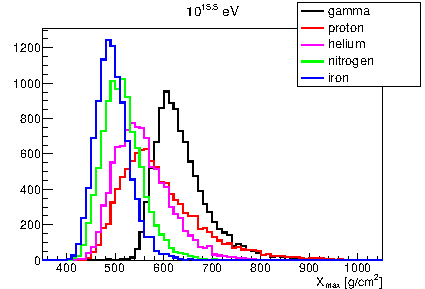
\includegraphics[width=1\textwidth]{pics/tunka_gamma_cr_diff.pdf}\\\small
    $X_{max}$ for various primaries at $E = 10^{15.5}$~eV for Tunka-133.
  \end{center}
\end{minipage}
\hfill
\begin{minipage}[c]{0.49\textwidth}
  \begin{center}
    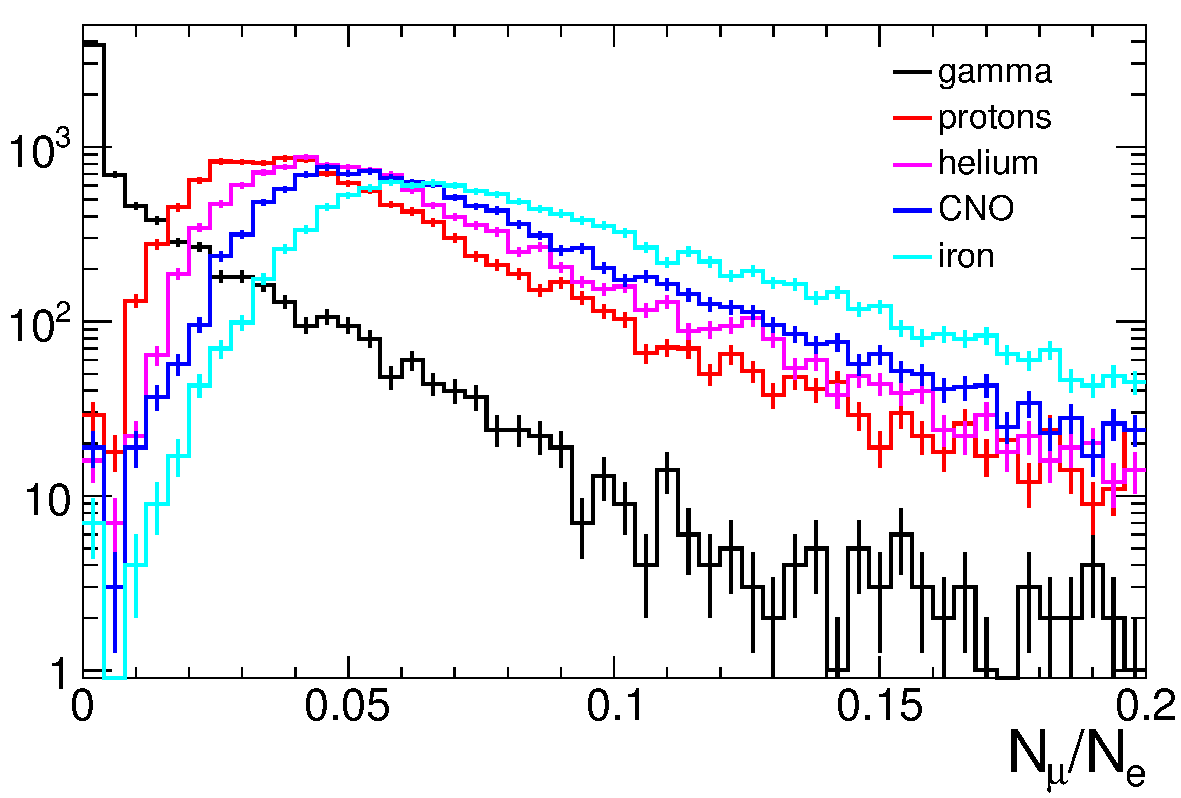
\includegraphics[width=1\textwidth]{pics/Nmu_Ne.pdf}\\\small
    $N_\mu / N_e$ for various primary CR components for KASCADE.
  \end{center}
\end{minipage}
\vspace{1ex}\small
\begin{itemize}
\setlength{\itemsep}{0pt}
\setlength{\parsep}{0pt}
\setlength{\parskip}{0pt}
  \item $\gamma$-proton separation can be performed quite well at KASCADE using electron-muon discrimination;
  \item The separation using $X_{max}$ at Tunka-133 is much more uncertain.
  \item It could be possible to select muon-poor showers using data from the Tunka-Grande setup.
\end{itemize}
\end{frame}
